\documentclass[11pt,a4paper
%,twocolumn
]{scrartcl}

% Support for UTF-8 and non-English letters require the following two
\usepackage[T1]{fontenc}
\usepackage[utf8]{inputenc}
% Font packages
\usepackage[default,defaultsans,oldstyle,proportional]{lato}
\usepackage[scaled]{beramono}
\usepackage{sfmath}
% Optimized justification via improved microtypography on character level
\usepackage{microtype}
\usepackage{ragged2e}
\usepackage[none]{hyphenat} % disable all hyphenation
\setlength{\emergencystretch}{3em} % allow extra hfill, needed if hyphenation disabled
%\overfullrule=1mm % mark overfull boxes
%\usepackage{showframe} % show edges of text areas
% Page layout
\usepackage[left=15mm,right=15mm,top=15mm,bottom=20mm,
   nohead,foot=10mm]{geometry}
% Page headers
\usepackage{scrlayer-scrpage}
\usepackage{lastpage}
% Page header
\KOMAoptions{headsepline=0pt,plainheadsepline=off}
\ihead*{}
\chead*{}
\ohead*{}
% Page footer
\KOMAoptions{footsepline=0pt,plainfootsepline=off}
\ifoot*{}
\cfoot*{Page \thepage{} of \pageref*{LastPage}}
\ofoot*{}
% Text layout
\KOMAoption{parskip}{never}
\newlength{\myparindent}
\newlength{\myparskip}
\setlength{\myparindent}{0pt}
\setlength{\myparskip}{5pt plus 1pt}
\setparsizes{\myparindent}{\myparskip}{0.1\linewidth plus 1fil}
\RedeclareSectionCommand[beforeskip=6pt,afterskip=3pt,afterindent=false]{section}
\RedeclareSectionCommand[beforeskip=6pt,afterskip=-0.5em,afterindent=false]{paragraph}
\RaggedRight
% SVN metadata
\usepackage[today,revrange,nofancy]{svninfo}
\svnInfo $Id$
% Graphics
\usepackage{graphicx}
% Colour definitions
\usepackage{xcolor}
\definecolor{secondary}{HTML}{435584}
% Floats
\usepackage{subcaption}
% Listings
\usepackage{listings}
\lstset{language=C, basicstyle=\small\ttfamily,
   aboveskip=0pt, belowskip=0pt}
\usepackage{upquote} % to use correct glyphs for single-quote in verbatim
% SI units
\usepackage{siunitx}
\sisetup{per-mode = symbol, detect-all = true}
% Hyperlinks
\usepackage[
   colorlinks=true,allcolors=secondary,breaklinks=true,
   bookmarks=true,unicode=true,bookmarksopen,bookmarksnumbered]{hyperref}
% Document-specific settings
\renewcommand\abstractname{Executive Summary}

% Document details
\title{Design Brief: Group 5}
\author{
   Gabriel Apap,
   Damjan Filipovic,
   Mark Mizzi
   }
\date{\svnMaxToday, Document v.\svnInfoMaxRevision}

\begin{document}

\maketitle

\abstract{%
   A Dual Tone Multi Frequency (DTMF for short) encoder is a technology used for devices or servers to communicate with other devices or servers over a standard analogue telephone line. This is mainly used for automated switchboards for calls; however, this is also used in dial up modems, call menus, remote control systems, telephone banking, and other applications. It functions by converting a possible 16 symbols on a keypad (1-9, A-D, * and \#) into a possible combination of 4 high frequencies (representing the keypad columns) and 4 low frequencies (representing the keypad rows). These frequencies are within the range of frequencies used to transmit the human voice allowing it to be transmitted over telephone lines as audible sounds that are however hard to reproduce by humans. The combination of signals is then received by the decoder and analysed to find which 2 signals make up the combination and thus which keypad symbol was pressed. \\[5mm]

   Implementing this on a microcontroller requires hardware interfacing, DTMF encoding techniques as well as low level microcontroller programming given that a microcontroller does not come pre-packaged with an operating system that abstracts low level system calls and basic hardware handling. Although this makes the job of the programmer harder it also gives them the opportunity to make their code very size and performance efficient by only including code that is specific to the task required. The design will make use of a display to show the user what keys they have pressed as well as to display any messages or errors. LEDs will also be used as indicators for different modes or statuses. The Digital to Analog Converter's output, which is used to turn the binary value from the program into an analogue electrical signal, is then connected to an amplifier so that a speaker can play the tone.



   }

\section{Introduction}
Write an introduction, explaining the purpose and background of this project.
Give a brief description of the game to be implemented.
Also include an overview of this document.

\section{System Design}

\subsection{System overview}

This section offers a brief overview of the designed system's features.

The system will make use of several I/O devices, including
\begin{enumerate}
   \item An LCD used to convey user input or settings options to the user.
   \item An indicator LED which turns on when the system is booted.
   \item A keypad input device used to choose between settings or to input DTMF symbols.
\end{enumerate}

On boot-up, the system will prompt the user to enter one of two operational modes: settings or normal mode.

In settings mode, the user is presented with numbered options which can be used to configure the system. 
The user's options are persisted to flash memory for use in normal mode.
The options available to the user will include:

\begin{enumerate}
   \item Inter-symbol spacing, i.e. the delay between two consecutive tones being produced.
   \item Symbol length, i.e. the duration for which a single tone is produced.
   \item Tone resolution. This setting affects the sampling frequency of the tone produced. A higher tone resolution produces a better quality tone, but is more computationally intensive.
   \item Reboot system. This saves the chosen options and resets the system.
\end{enumerate}

When the system enters normal mode, options are loaded from flash memory, and the system behaves as a DTMF encoder, 
producing tones when the user presses keys.

\subsection{System architecture}

To implement these features while adhering to good seperation of concerns, the system must make use of several software components.
The proposed software components are shown in Figure \ref{fig:software_components}.

\begin{figure}
   \centering
   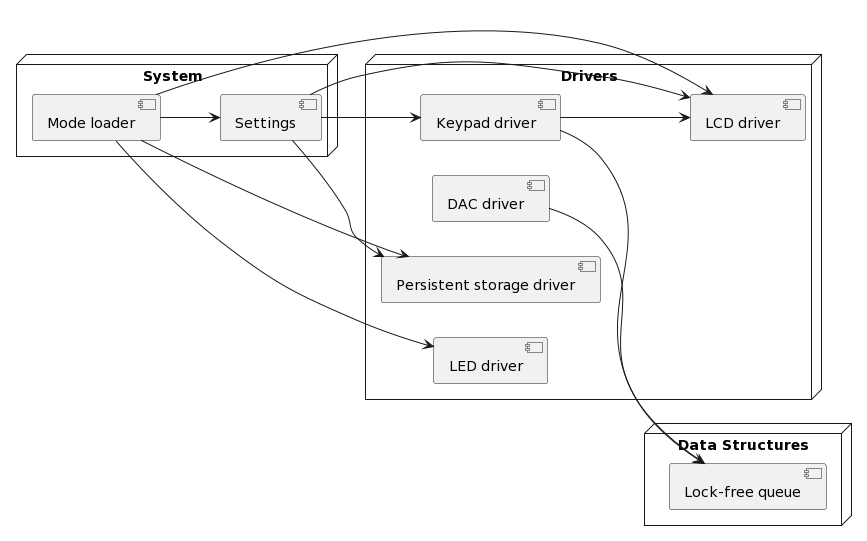
\includegraphics[width=0.75\textwidth]{software_components}
   \caption{Software components proposed for the system, grouped by functionality. Arrows between components indicate caller-callee dependencies.}
   \label{fig:software_components}
\end{figure}

Not shown in this figure is the use of several global variables to store the state of the system. These include:

\begin{enumerate}
   \item A global, thread-safe flag which indicates whether a tone is being generated.
   \item A global counter used to keep track of tone generation in between interrupt handler invocations (see below).
   \item A global C \verb!struct! holding user configuration of the system. 
      In normal mode, this is loaded from flash memory, and should be read-only.
      In settings mode, the configuration is loaded from flash memory or initialized with sane defaults depending on whether the user has already 
      configured the system. In this mode, the \verb!struct! can be modified.
   \item A global lookup-table containing samples of the $\sin$ function. This is loaded in normal mode, and should be read-only.
\end{enumerate}

It is also worth noting that the lock-free queue indicated in the design is globally allocated, and is accessed by several ``threads'' of execution.

The responsibilities and features of each of the software components indicated in the figure will now be described.

The \textbf{mode loader} is the entry point of the system. It turns on the indicator LED (through the use of the LED driver), and presents the user with options
for choosing between settings mode or normal mode (through the LCD driver). It must also process any key press which indicates the user's choice 
(through the keypad driver), and load the code for settings or normal mode (through a function call).

The \textbf{settings} component will contain the code for settings mode. It must present the user with options for configuring the system (through the use of the
LCD driver), and process the user's choice (through the use of the button matrix driver). When the user chooses to re-boot the system, it must also persist the
chosen configuration to flash memory (through the use of the persistent storage driver).

The \textbf{DAC driver} is central to system operation, as it contains functions which generate the DTMF tones. The module should provide a function which, 
given a symbol, enables a timer interrupt handler (depending on what tone is to be produced) and sets the timer duration to the sampling frequency of the tone.

The module should also implement 16 timer interrupt handlers (one for each tone) which can produce tone samples and 
drive the DAC when a tone is being generated. The interrupt handlers will be similar in behaviour, and will share a lot of their code. However
there are two benefits in having an interrupt handler for each tone. Firstly, there is no need to keep track of which tone is being generated in between invocations
of the interrupt handler. This reduces the amount of global state used by the system. Secondly, specializing the code depending on the tone to be produced allows the
compiler to aggressively optimize the handlers in question, e.g. applying constant division optimization.

The behaviour of each interrupt handler is shown in the control flow diagram in Figure \ref{fig:tone_interrupt_cfd}. Note the ``bootstrapping'' behaviour of tone
generation. When an interrupt handler detects that tone generation is done, it checks the queue for the next symbol whose tone is to be generated. 
If there is one, it pops it off the queue, and sets a timer according to the inter-symbol spacing. It also enables a handler for the timer interrupt which
starts off the next tone's interrupt handler. Note that the check and pop from the queue must be done atomically to avoid data races.

\begin{figure}
   \centering
   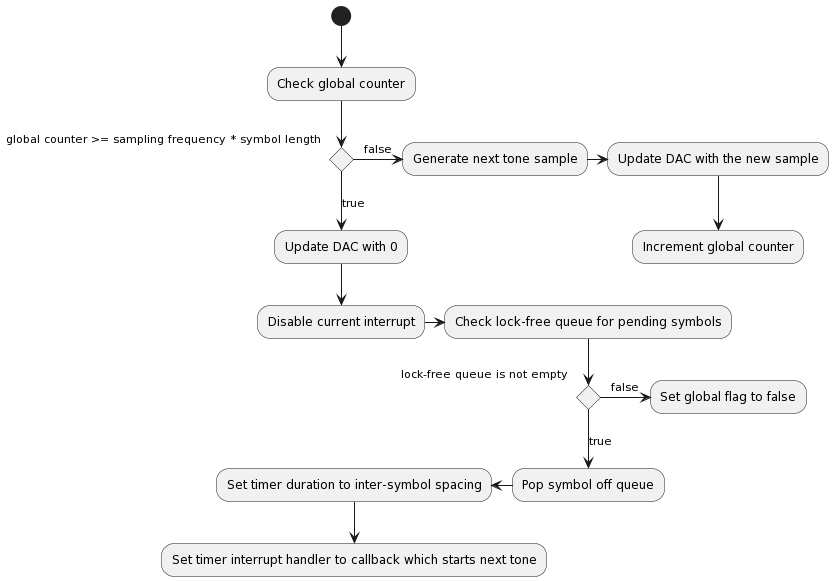
\includegraphics[width=0.75\textwidth]{tone_interrupt_cfd}
   \caption{Control flow diagram illustrating behaviour of tone-generating interrupt handlers}
   \label{fig:tone_interrupt_cfd}
\end{figure}

The \textbf{keypad driver} component provides an abstraction layer over the keypad. It must implement a single polling cycle (as a function) for use in other modules.

In addition, it must implement a method that whilst running the polling cycle, performs the following actions immediately on detection of a key press:
\begin{enumerate}
   \item It immediately outputs the DTMF symbol detected to the LCD screen.
   \item It checks if there is a tone interrupt handler enabled. This can be done by atomic test and set on the global flag.
   \item If there is no tone interrupt handler enabled, it takes the symbol detected, and enables a tone-generating interrupt handler to generate its tone 
      (using a method in the DAC driver).
   \item If there is already a tone interrupt handler enabled, it pushes the DTMF symbol onto the output queue.
\end{enumerate}
This method will be used in normal mode to process key presses.

The \textbf{persistent storage driver} provides an abstraction layer over the flash memory. It provides functions to serialize and deserialize the C structs 
which need to be stored into a byte stream, and allows for loading or storing serialized data from/to flash memory. The use of a wear leveling algorithm when storing data
is essential to prevent the flash memory from degrading quickly\cite{silberschatz2018operating}.

The \textbf{LED driver} provides methods to turn the indicator LED on or off.

The \textbf{LCD driver} provides an abstraction layer over the LCD screen. It must implement methods which allow a DTMF symbol or a C string to be encoded and
displayed on the LCD.

The \textbf{lock-free queue} is a globally allocated thread-safe data structure. It needs to support the following thread-safe (atomic) operations:
\begin{enumerate}
   \item Enqueue a DTMF symbol.
   \item Check if queue is empty and dequeue. This must be one atomic operation.
\end{enumerate}

\subsection{How the polling method is invoked}

There are several ways in which the polling cycle procedure that processes user input in normal mode (described above) can be executed.

The simplest method is to run the procedure in application mode, with a set period of busy waiting in between invocations of the method to avoid spurious input.
(A human user will keep a key pressed for several clock cycles.)

A more sophisticated option is to run the procedure as an interrupt handler for a timer interrupt, with the timer duration set to avoid spurious input. In this
version, the processor has no application code to run and can be put in sleep mode in between interrupt invocations. While more efficient than the busy-waiting
approach, this method can still invoke the interrupt handler when there is no input to process.

A final, more efficient approach is to have a keypad-driven interrupt handler. In this approach, the columns of the keypad are set high, and pressing any key
triggers a pin interrupt. The interrupt handler then invokes the polling method to handle the key pressed.

Each of these design choices is more sophisticated than the one before it, while re-using much of the same code. 
The plan is hence to implement each of these designs in turn. When one implementation has been successfully tested, the team will move on to implementing a more
sophisticated design.

\section{Management}
Include a time plan.
Show task dependencies.
How are these going to be managed?

\section{Closure}

\bibliographystyle{ieeetr}
\bibliography{references}

\end{document}
